% Это основная команда, с которой начинается любой \LaTeX-файл. Она отвечает за тип документа, с которым связаны основные правил оформления текста.

%Article
\documentclass[14pt]{extarticle}

% Здесь идет преамбула документа, тут пишутся команды, которые настраивают LaTeX окружение, подключаете внешние пакеты, определяете свои команды и окружения. В данном случае я это делаю в отдельных файлах, а тут подключаю эти файлы.

% Здесь я подключаю разные стилевые пакеты. Например возможности набирать особые символы или возможность компилировать русский текст. Подробное описание внутри.
\usepackage{packages}

% Здесь я определяю разные окружения, например, теоремы, определения, замечания и так далее. У этих окружений разные стили оформления, кроме того, эти окружения могут быть нумерованными или нет. Все подробно объяснено внутри.
\usepackage{environments}

% Здесь я определяю разные команды, которых нет в LaTeX, но мне нужны, например, команда \tr для обозначения следа матрицы. Или я переопределяю LaTeX команды, которые работают не так, как мне хотелось бы. Типичный пример мнимая и вещественная часть комплексного числа \Im, \Re. В оригинале они выглядят не так, как мы привыкли. Кроме того, \Im еще используется и для обозначения образа линейного отображения. Подробнее описано внутри.
\usepackage{commands}

% Пакет для титульника исследовательского проекта
\usepackage{titlepage}

% Здесь задаем параметры титульной страницы
\setToProgram
\setTitle{Продвинутый 3D renderer}
\setGroup{196}
%сюда можно воткнуть картинку подписи
%\setStudentSgn{\includegraphics[scale=0.2]{signature.png}}
\setStudent{Смородинов Александр Андреевич}
% \setStudent{[Данные удалены]} % TODO: не забыть вернуть всё как было
%\setStudentDate{03.06.2021}
\setAdvisor{Трушин Дмитрий Витальевич}
\setAdvisorTitle{Доцент, кандидат физико-математических наук}
%\setAdvisorAffiliation{ФКН НИУ ВШЭ}
%\setAdvisorDate{}
%\setGrade{}
%сюда можно воткнуть картинку подписи
%\setAdvisorSgn{}
\setYear{2022}

\usepackage{dejavu}
% \usepackage{kpfonts}

% С этого момента начинается текст документа
\begin{document}

% Эта команда создает титульную страницу

\makeTitlePage

% Здесь будет автоматически генерироваться содержание документа
\renewcommand*\contentsname{Оглавление}
\tableofcontents


% Данное окружение оформляет аннотацию: краткое описание текста выделенным абзацем после заголовка
\section{Аннотация}
На сегодняшний день технологии отрисовки трёхмерных сцен используются во многих сферах нашей жизни: в 3D моделировании и анимации, в компьютерных играх и 3D/VR симуляциях. Первые статьи по данной теме были опубликованы ещё в 60х-70х годах 20 века, и с тех пор было проведено огромное количество исследований и работ в сфере 3D рендеринга. 

Цель данной работы - изучить и реализовать ряд важнейших алгоритмов 3D рендеринга. 

На втором курсе в рамках программного проекта было реализовано с нуля приложение, позволяющее пользователю взаимодействовать с трёхмерной сценой, задавать различные режимы отрисовки для объектов сцены, менять параметры освещения, источников света, камеры и экрана в реальном времени.

В рамках данной курсовой работы в приложение была добавлена поддержка различных продвинутых алгоритмов отрисовки: normal mapping, parallax mapping, HDR, bloom, shadow mapping, отрисовка полупрозрачных объектов, deferred shading, SSAO, а также была улучшена производительность.

\section*{Abstract}
Nowadays 3D rendering algorithms are used in many parts of our lives: 3D modeling and animation, computer games and 3D/VR simulations. First articles on this topic were published in the sixties and seventies of the 20th century, and since then a large number of studies have been carried out on this topic.

The goal of this paper is to study and implement some of the main 3D rendering algorithms.

In the second year as part of a program project, an application was developed from scratch that allows user to interact with 3D scene, set different modes of rendering for scene objects, change parameters of lighting, light sources, camera and screen in real time.

As part of this paper, support for advanced algorithms such as normal mapping, parallax mapping, HDR, bloom, shadow mapping, rendering of transparent objects, deferred shading and SSAO, was added to the application, and performance was also improved.

\subsection{Ключевые слова}
Программный 3D рендеринг, shadow mapping, normal mapping, parallax mapping, HDR, bloom, deferred shading, SSAO, C++, SFML, glm, imgui, stb\_image.

\section{Введение}

\subsection{Постановка задачи}
\subsubsection{Цели}
Основная цель проекта - это изучение и реализация алгоритмов, использующихся в компьютерной графике, на которых основаны большинство программ 3D моделирования, 3D игр, 3D/VR симуляторов и других приложений, имеющих какое-либо отношение к трёхмерной графике. 
\subsubsection{Задачи}
Основные задачи:
\begin{itemize}
	\item Изучить и реализовать продвинутые алгоритмы 3D рендеринга (в секции с описанием полученных результатов будет конкретный список).
	\item Интегрировать реализацию продвинутых алгоритмов в существующую базовую версию 3D рендерера (в интерактивное приложение).
	\item Изложить теоретические основы реализованных алгоритмов, описать детали их реализации, написать сопроводительную документацию к коду и протестировать его.
\end{itemize}

\subsection{Актуальность и значимость}
3D рендеринг - это активно развивающаяся и относительно молодая область компьютерной графики, и результаты исследований в данной сфере часто находят применение в 3D анимации, моделировании, 3D/VR симуляторах, компьютерных играх и других приложениях.

Важной особенностью описываемой в данной работе реализации является тот факт, что в проекте не используются такие известные API для работы с компьютерной графикой как OpenGL, DirectX, Vulcan и др. Это означает, что весь рендеринг происходит исключительно на CPU (так называемый software rendering). 

Данный подход имеет ряд своих преимуществ и недостатков, по сравнению с GPU rendering-ом:

Преимущества:
\begin{itemize}
	\item Работает на всех устройствах, независимо от наличия видеокарты (в том числе микроконтроллерах и других встроенных системах).
	\item Также не нужно требовать от видеокарты пользователя поддержки конкретной версии API (например OpenGL 3.3).
	\item На всех устройствах одно и то же приложение работает одинаково, нет уязвимости к багам реализации API.
	\item У разработчика software renderer-а есть полный контроль над реализацией. Добавлять новые функции в рендерер, изменять существующие алгоритмы, исправлять баги в реализации в разы проще и быстрее, чем при использовании сторонних решений.
	\item С образовательной точки зрения, самостоятельная реализация 3D рендерера с нуля даёт намного более глубокое понимание работы алгоритмов 3D рендеринга, чем просто использование некоторой готовой библиотеки.
\end{itemize}

Недостатки:
\begin{itemize}
	\item Главный недостаток - скорость. Видеокарты намного лучше справляются с множеством хорошо распараллеливаемых вычислений, чем процессоры. Они специально для этого и проектировались. Разница в скорости очень сильно зависит от конкретной видеокарты и конкретного приложения, но может составлять несколько порядков.
	\item С точки зрения разработчика - нужно всё писать с нуля самому, а не использовать API (хотя также есть и уже написанные библиотеки).
\end{itemize}

Реализованный в данной работе 3D рендерер, так как является программным, практически не имеет шансов соперничать с существующими аппаратными рендерами в производительности.

Тем не менее в случаях, когда производительность не так важна, но необходима кроссплатформенность и отсутствие большого количества внешних зависимостей, реализованный 3D рендерер может быть полезен в качестве библиотеки отрисовки, так как он поддерживает не только базовые, но и продвинутые алгоритмы рендеринга.

Также, данный проект будет полезен в качестве примера реализации программного 3D рендерера на C++, поддерживающего продвинутые алгоритмы, для тех, кто интересуется компьютерной графикой и C++.

Работа также значима лично для автора статьи, как возможность изучить алгоритмы 3D рендеринга и реализовать их на практике.

\subsection{Полученные результаты}
\subsubsection {Репозиторий}
Репозиторий проекта: ~\cite{3dRenderer}

\subsubsection{Реализованные продвинутые алгоритмы}
\begin{enumerate}
	\item Отображение нормалей (normal mapping).
	\item ''Параллакс'' отображение (parallax mapping).
	\item HDR, tone mapping, gamma correction.
	\item Bloom.
	\item Рендеринг прозрачных объектов.
	\item Shadow mapping.
	\item Отложенное освещение и затенение (deferred shading).
	\item Screen space ambient occlusion (SSAO).
\end{enumerate}

\subsubsection{Функциональные требования к результату}
Результат проекта - интерактивное приложение, доступное на ОС windows / linux, в котором пользователь может:
\begin{itemize}
	\item Просматривать различные 3D сцены, управляя камерой с клавиатуры.
	\item Настраивать параметры сцены.
	\item Открывать и добавлять в сцену 3D объекты, сохранённые в различных форматах (на данный момент реализована загрузка простейших 3D моделей в формате wavefront obj ~\cite{obj}).
\end{itemize}
\subsubsection{Нефункциональные требования к результату}
\begin{itemize}
	\item Язык программирования - C++ (стандарт C++17).
	\item Используемые библиотеки (статическая линковка):
	\begin{itemize}
		\item glm 0.9.9 ~\cite{glm}.
		\item SFML 2.5.1 ~\cite{sfml}.
		\item ImGui v1.83 ~\cite{imgui}.
		\item stb\textunderscore image 2.26 ~\cite{stb}.
	\end{itemize}
	\item Система контроля версий - git.
	\item Линтер/форматтер - clang format, настройки основаны на google codestyle.
	\item Для сборки проекта используется IDE Microsoft Visual Studio 2019.
\end{itemize}

\subsection{Новизна и полезность полученных результатов}
С теоретической точки зрения все реализованные алгоритмы являются достаточно известными и применяются во многих 3D рендерерах. Например, большая часть из них описана на сайте ~\cite{learnopengl}, а также в книгах ~\cite{LRN} и ~\cite{Math3d}. Поэтому теоретической значимости и новизны в данном проекте практически нет.

Но, с практической точки зрения, как далее будет показано, аналогов программного 3D рендерера на C++, поддерживающих все перечисленные выше продвинутые алгоритмы отрисовки, в открытом доступе довольно мало, если они вообще есть (по крайней мере автор прямого аналога не нашёл), и в этом плане работа обладает некоторой новизной. Обоснование практической полезности программных 3D рендереров было приведено выше.

Так как проект программный, такое положение вещей кажется достаточно естественным (малая теоретическая полезность, но существующая практическая полезность).

\subsection{Структура работы}
В секции 3 приведён обзор аналогов.
В секции 4 приведено краткое описание реализованных алгоритмов.
В секции 5 описываются особенности реализации приложения.
Секция 6 - заключение отчёта по курсовой работе.
После секции 6 идёт список источников.

\section{Обзор аналогов}
Существует множество реализаций программных 3D рендереров. Во многих институтах, где читают лекции по 3D графике реализация 3D рендерера может являться домашним заданием которое выполняют студенты. Также многие разработчики реализуют 3D рендерер для того, чтобы изучить различные алгоритмы 3D рендеринга, в качестве так называемого pet-project-а.

За исключением данных примеров, программные 3D рендереры на данный момент применяются достаточно редко, в основном из-за их низкой производительности по сравнению с аппаратными 3D рендерерами.

\subsection{Mesa}
Это не совсем аналог данного проекта, но Mesa - ~\cite{mesa} содержит программную (software rendering) реализацию OpenGL 3.1. Так что можно с использованием Mesa пользоваться OpenGL (и рядом других API) даже на устройствах, не имеющих GPU (также Mesa реализует набор видеодрайверов для различных GPU).

На устройствах с дистрибутивами GNU/Linux, *BSD и другими ОС Mesa является основой графического стека, так как Mesa - это свободная реализация основных графических API.

Из-за такого широкого распространения было бы немного неправильно вообще не упомянуть данное решение, но как уже было написано выше - это не совсем аналог данного проекта, поэтому сравнивать их между собой довольно сложно.

\subsection{Другие аналоги}
Так как в интернете в открытом доступе существует большое количество реализаций программного 3D рендеринга, то все их проанализировать не получится, поэтому будет приведён только анализ наиболее популярных по количеству звёзд на гитхабе решений. (метрика популярности довольно произвольная, но нужно же было как-то отсортировать решения). Поиск проектов на гитхабе был по топику software-rendering (полный список - ~\cite{analogsList}).


\begin{enumerate}
	\item ssloy/tinyrenderer ~\cite{renderer1} Отличный проект, весь код занимает примерно 500 строчек. Но реализовано не так много алгоритмов 3D рендеринга (например нет клиппинга). Вообще проект в основном носит образовательный характер, и в этом плане там очень хорошие уроки на вики странице.
	\item zauonlok/renderer ~\cite{renderer2} Тоже интересный проект, написан на C89, реализовано довольно много алгоритмов, но более продвинутые техники также не реализованы.
	\item kosua20/herebedragons ~\cite{renderer3} Не совсем корректно считать этот проект аналогом, так как это не software рендерер, а наоборот, реализация одной сцены с помощью разных графических API. Интересно то, что также есть реализации сцены на платформах, где никаких API для 3D графики нет (например для PICO-8 и Nintendo Game Boy Advance). На таких платформах используются различные способы обойти аппаратные ограничения.
	\item skywind3000/mini3d ~\cite{renderer4} Небольшой (700 строк) 3D рендерер на c. Не реализованы почти никакие дополнительные / продвинутые алгоритмы.
	\item ssloy/tinyraycaster ~\cite{renderer5} Как видно из названия, это рейкастер, а не полноценный 3D рендерер, поэтому тоже не очень корректный пример.
	\item skywind3000/RenderHelp ~\cite{renderer6} Ещё один довольно простой 3D рендерер на C++.
	\item Angelo1211/SoftwareRenderer ~\cite{renderer7} Один из самых интересных проектов из всего списка. Реализовано довольно много продвинутых алгоритмов. Тем не менее, есть несколько проблем с сглаживанием и ''Муаровым эффектом'' в некоторых сценах, а также есть нереализованные алгоритмы (из списка реализованных в данном проекте).
	\item martinResearch/DEODR ~\cite{renderer8} Дифференцируемый 3D рендерер на c. Какая-то классная штука для ML. Не уверен, часто ли данную библиотеку используют в других областях.
\end{enumerate}

Бонусные аналоги (не из списка выше, по крайней мере не из топа по звёздам)
\begin{enumerate}
	\item bytecode77/fastpix3d ~\cite{renderer9} Данный 3D рендерер показывает довольно хорошие показатели по производительности. Хотя в примерах используются не очень детализированные модели и текстуры в не очень высоком разрешении, производительность не может не впечатлять, учитывая, что это software рендерер. Каких-то очень продвинутых алгоритмов не реализовано, хотя есть поддержка освещения и теней.
	\item Dawoodoz/DFPSR ~\cite{renderer10} В данном проекте применены очень интересные идеи. Библиотека предназначена для изометрических игр/сцен, и если использовать тот факт, что объекты всегда будут видны только с одного ракурса, то можно ''запечь'' (pre-render, bake) 3D модель в три текстуры - diffuse, normal, height, а дальше работать с моделью как с одним прямоугольником (причём ориентированным в пространстве камеры вдоль координатных осей). Это очень сильно снижает необходимое количество вычислений на процессоре и позволяет отрисовывать достаточно сложные изометрические сцены в реальном времени.
\end{enumerate}

Как можно видеть, довольно мало проектов из перечисленных выше реализуют какие-то продвинутые алгоритмы 3D рендеринга. 

Вывод: реализованный проект имеет практическую значимость и имеет малое количество аналогов по функциональным возможностям. 

Также можно дополнительно отметить, что в реализованном приложении есть UI для редактирования сцены и параметров отдельных объектов, тогда как большинство перечисленных аналогов поддерживают только отображение статичных сцен (без возможности их редактирования прямо в приложении).

\section{Краткое описание реализованных алгоритмов}
Далее будет представлено очень краткое описание реализованных алгоритмов. Более подробную информацию можно найти в книгах ~\cite{LRN}, ~\cite{Math3d} и на сайте ~\cite{learnopengl} (здесь описание алгоритмов объясняется наверное наиболее доступно), если читатель захочет более глубоко ознакомиться с тематикой проекта. Предполагается, что с базовыми понятиями 3D рендеринга читатель уже знаком. Если это не так, то можно например прочитать отчёт по курсовой работе прошлого года ~\cite{year2paper}.

\subsection{HDR}
Большинство мониторов способны отображать только цвета, каждый (r, g, b) компонент которых лежит в интервале от 0 до 1 (или от 0 до 255, если компонент задаётся одним байтом, а не числом с плавающей точкой). Поэтому в большинстве графических API, в частности OpenGL, по умолчанию отрисовка производится в буфер, в котором все компоненты также ограничены интервалом $[0, 1]$. В базовой версии программного 3D рендерера буфер также поддерживает только цвета с ограниченными компонентами. 

При этом если в 3D сцене при вычислении цвета пикселя получается так, что его компоненты превосходят 1, то по умолчанию величины компонент просто уменьшают до 1 (например $(1.2, 0.3, 1.7) \Rightarrow (1, 0.3, 1)$). Такое преобразование цвета с произвольными компонентами в цвет с ограниченными компонентами называется tone mapping. Изначально цвет у нас задаётся без ограничений, то есть в HDR (High Dynamic Range), и мы преобразуем его в LDR (Low Dynamic Range) цвет (компоненты от 0 до 1).

Наивное clamp преобразование (когда мы просто ограничиваем величины больше 1 единицей) приводит к тому, что мы теряем информацию о цвете ярких фрагментов сцены. Большие участки сцены могут например просто все быть отрисованы одним белым цветом ($(1, 1, 1)$), что выглядит не очень красиво.

Есть множество распространенных tone mapping функций, которые обеспечивают различный баланс детализации тёмных и ярких участков сцены.

Например преобразование exposure tone mapping: $1 - \exp(-x \cdot \varepsilon)$, где $\varepsilon$ - настраиваемый параметр (выдержка), в зависимости от которого сцена будет отрисована либо светлее, либо темнее.

Часто бывает полезно не сразу делать tone mapping внутри шейдера, а отрисовать сцену в HDR буфер, использовать его (например применить ещё bloom), и только потом преобразовать HDR буфер в LDR, с применением tone mapping.

\subsection{Bloom}
Данная техника в большинстве случаев применяется вместе с HDR. Основная идея состоит в том, чтобы добавить ярким источникам света эффект ''свечения'': вокруг данных источников свет ''проникает'' в другие пиксели (это выражается в том, что пиксели вокруг ярких источников света в небольшом радиусе сами становятся ярче и частично окрашиваются в цвет источника). Если использовать данный эффект в разумных количествах, то это позволяет создавать интересные сцены и значительно улучшить качество освещения сцены.

Реализуется bloom следующим образом:
\begin{enumerate}
	\item Отрисовываем сцену в HDR буфер.
	\item Выделяем из HDR буфера яркие пиксели (например с яркостью > 1) и копируем их во вспомогательный буфер (изначально вспомогательный буфер полностью чёрный).
	\item Применяем какой-нибудь алгоритм размытия (например Гауссовское размытие, его можно эффективно реализовать как горизонтальное + вертикальное размытие). Для вычисления Гауссовского размытия нужно для каждого пикселя вычислить среднее взвешенное цветов соседних (например в квадрате $N\times N$) пикселей, при этом в качестве весов используется функция Гаусса. Благодаря свойству, что двумерное гауссовское размытие можно представить как последовательное одномерное горизонтальное и вертикальное размытие (размытие отдельных строк и столбцов), можно значительно снизить количество вычислений (из квадратичного по $N$ до линейного). 
	\item Прибавляем к оригинальному буферу вспомогательный.
	\item Делаем tone mapping.
\end{enumerate}

Рис. \ref{fig:bloom} - пример сцены, отрисованной без HDR, с HDR и с bloom-ом. (возможно была выбрана не лучшая сцена для демонстрации данного эффекта)

\begin{SCfigure}[0.5][h]
	\label{fig:bloom}
	\caption{Сравнение обычной сцены, сцены с HDR и сцены с bloom.}
	\includegraphics[width=0.6\textwidth]{bloom.png}
\end{SCfigure}

\subsection{Отрисовка полупрозрачных объектов, blending}
Сквозь полупрозрачные объекты можно видеть объекты за ними, но при этом цвет этих объектов также изменяется в зависимости от цвета полупрозрачного объекта, который расположен перед ними. Этот эффект в 3D рендеринге называется blending (смешение), так как цвета различных объектов ''смешиваются''. 

Если поддержать в 3D рендерере blending, то это позволит отрисовывать сцены с полупрозрачными объектами. Чтобы реализовать blending, нужно просто перед тем, как записывать пиксель в буфер вызывать специальную $blend$ функцию, которая принимает цвет текущего пикселя в буфере ($destination$), а также цвет пикселя, который мы хотим записать ($source$). И в буфер мы уже будем записывать не $source$, а $blend(destination, source)$ - результат $blend$ функции. 

Также необходимо каким-то образом упорядочить пиксели при их отрисовке по уменьшению глубины, так как функция $blend$ в общем случае не является коммутативной и от порядка попадания пикселей в буфер будет зависеть итоговый результат. При этом ''правильный'' порядок применения $blend$ функции - это именно от дальних пикселей к ближним. Например, самые близкие к камере пиксели полупрозрачных объектов должны быть аргументами $blend$ только один раз, и только в качестве $source$, иначе результат будет выглядеть некорректно.

В реализованном 3D рендерере сортировка пикселей производится довольно наивно - сортируются только отдельные треугольные грани объектов, при этом расстояние считается от камеры до центра треугольников. Для многих сцен такой подход работает достаточно неплохо (без артефактов), но существуют случаи, когда он будет производить некорректные результаты (обычно когда два треугольника находятся близко друг к другу).

Одной из возможных альтернатив было бы хранить в буфере цветов для каждого пикселя целый список цветов (то есть не использовать depth test для полупрозрачных фрагментов, и сохранять все такие фрагменты). Минусом такого решения было бы достаточно высокое потребление памяти (в теории неограниченное, в зависимости от сложности сцены и потенциально растущее достаточно быстро), и также скорость отрисовки, из-за сложности такого подхода. Но в теории, такой вариант реализации тоже возможен, хотя на практике он встречается довольно редко (впрочем, то же самое можно сказать и о программных рендерерах), в частности из-за того, что большинство видеокарт не поддерживают такие неограниченные по глубине и по сути трёхмерные буферы.

Проблема отрисовки полупрозрачных объектов является достаточно нетривиальной, какого-то однозначно общепринятого решения кажется нет, поэтому применённый подход, учитывая свою простоту, в целом является неплохим.

Рис. \ref{fig:transp} - отрисованная сцена с полупрозрачными объектами.

\begin{SCfigure}[0.5][h]
	\label{fig:transp}
	\caption{Сцена с полупрозрачными объектами.}
	\includegraphics[width=0.6\textwidth]{transparent.png}
\end{SCfigure}

\subsection{Shadow mapping}
Данный алгоритм применяется для отрисовки теней от направленных источников света (то есть располагающихся настолько далеко, что испускаемые ими лучи можно считать параллельными, например в некоторых случаях можно рассматривать солнце как такой источник).

Основная идея состоит в том, что сначала мы отрисовываем всю сцену с камерой расположенной в некоторой позиции, так чтобы сцена помещалась на экран (эту позицию можно считать источником, хотя и предполагается, что источник расположен бесконечно далеко), направленной так же, как и источник света. В тени будут находиться все фрагменты, которые не попали в итоговый буфер (то есть провалившие проверку на глубину - depth check), при отрисовке сцены со стороны источника света. Действительно, если фрагмент не попал в буфер, то это означает, что есть какой-то другой фрагмент, находящийся ближе к камере, чем он, то есть загораживающий его от света. Рис. \ref{fig:shadow1} демонстрирует эту идею в двумерном случае.

\begin{SCfigure}[0.5][h]
	\label{fig:shadow1}
	\caption{Освещённые и затененные фрагменты сцены, источник - ~\cite{shadow1}.}
	\includegraphics[width=0.6\textwidth]{shadowmapping1.png}
\end{SCfigure}

После того, как мы отрисовали сцену с позиции источника света, у нас есть буфер цветов, который нам не пригодится, и буфер глубины, который дальше будет нужен, назовём его shadow map (или depth map). Заметим (достаточно тривиальный факт), что в буфере глубины для каждого фрагмента (пикселя) хранится минимальное расстояние (по оси $z$) от камеры до некоторого объекта сцены.

Теперь необходимо отрисовать сцену с исходной позиции камеры, и при этом уметь определять по фрагменту, находится он в тени, или нет. 

Позиция фрагмента задаётся в пространстве мира (world space - глобальные координаты), сначала её необходимо преобразовать в пространство источника света - то есть умножить на view матрицу из прошлого шага, когда сцена отрисовывалась с позиции источника света. 

Затем нужно из пространства источника света перевести координаты в экранные (то есть применить матрицу проекции, использующуюся на прошлом шаге). 

Теперь мы получили нормализованные координаты $x, y$, которые можно использовать как текстурные координаты при обращении к буферу глубины (shadow map) и с помощью него получить глубину $z_0$ фрагмента, находящегося ближе всего к источнику света. Также у нас есть $z$ координата - это глубина текущего фрагмента, относительно источника света. 

Если $z > z_0$, то есть объект ближе к источнику света, чем текущий фрагмент, а значит текущий фрагмент находится в тени (утверждение верно в обе стороны). 

Если мы знаем, что фрагмент находится в тени, то можно в шейдере умножить посчитанное значение цвета фрагмента на константу $<1$, или визуализировать это как-то по другому.

Рис. \ref{fig:shadow2} показывает, как лучи света соотносятся с значениями глубины, сохранёнными в depth map (shadow map), и как производится преобразование позиции фрагмента в пространство источника света.

\begin{SCfigure}[0.5][h]
	\label{fig:shadow2}
	\caption{Буфер глубины, преобразование в пространство источника света, источник - ~\cite{shadow2}.}
	\includegraphics[width=0.6\textwidth]{shadowmapping2.png}
\end{SCfigure}

Рис. \ref{fig:shadow3} - пример сцены, отрисованной с применением shadow mapping-а.

\begin{SCfigure}[0.5][h]
	\label{fig:shadow3}
	\caption{Shadow mapping.}
	\includegraphics[width=0.6\textwidth]{shadows.png}
\end{SCfigure}

\subsection{Карта нормалей (normal mapping)}
Для обеспечения более реалистичного и детализированного рендеринга модели на экране часто применяются карты нормалей. 

Большинство поверхностей в реальном мире содержат множество неровностей и никогда не являются плоскими на 100 процентов. В 3D сценах же наоборот, все объекты состоят из плоских треугольников, которые можно достаточно легко заметить, если они довольно большие и их не очень большое число.

В большинстве моделей освещения участвуют векторы нормалей, и для всей плоскости вектор нормали один и тот же. Но если для каждого фрагмента плоскости использовать вектор нормали, заданный в отдельной текстуре (карте нормалей), то с точки зрения освещения каждый фрагмент уже не будет иметь один и тот же вектор нормали, и это создаст иллюзию, что поверхность уже не является плоскостью и содержит множество неровностей (так как она освещается не так, как освещалась бы плоскость). 

Такой приём позволяет значительно увеличить реалистичность моделей, добавить им больше деталей и создать иллюзию ''глубины'' для плоскостей.

После получения вектора нормали из карты нормалей его нужно перевести в пространство мира из так называемого касательного пространства (tangent space) треугольника, который мы отрисовываем (карта нормалей строится для поверхности, ориентированной вдоль плоскости XOY, перпендикулярно оси Z, но отрисовываемый треугольник в сцене может иметь произвольную ориентацию). Это делается с помощью $TBN$ матрицы ($tangent$, $bitangent$, $normal$ - это базис касательного пространства, записанный в пространстве мира, см. рис.  \ref{fig:tbn}), которая вычисляется в вершинном шейдере. 

\begin{SCfigure}[0.5][!h]
	\label{fig:tbn}
	\caption{TBN вектора, источник - ~\cite{tbn}.}
	\includegraphics[width=0.3\textwidth]{tbn.png}
\end{SCfigure}


Если умножить вектор в касательном пространстве на матрицу $TBN$ слева, то мы получим координаты данного вектора в пространстве мира (вектора $(1,0,0), (0,1,0), (0,0,1)$ перейдут в вектора $tangent, bitangent, normal$, при этом можно считать, что плоскость проходит через начало координат в пространстве мира, так как нас интересует только вектор нормали в пространстве мира, а он не зависит от положения плоскости, а только от её ориентации).

Рис. \ref{fig:normal} - отрисованный куб (хотя и видна только одна грань) без и с normal mapping-ом.

\begin{SCfigure}[0.5][h]
	\label{fig:normal}
	\caption{Blinn-Phong шейдер без и с normal mapping-ом.}
	\includegraphics[width=0.6\textwidth]{normal.png}
\end{SCfigure}

\subsection{Parallax mapping}
Идея похожа на normal mapping, но здесь вместо карты нормалей используется карта смещения (displacement map). В этой текстуре задаётся смещение каждого фрагмента треугольника по глубине. С помощью parallax mapping-а по карте смещения, текущим текстурным ($uv$) координатам, и направлении вдоль которого мы смотрим на фрагмент ($viewPos - fragPos$) мы определяем новые текстурные ($uv$) координаты (намного более детально этот процесс описывается в ~\cite{learnopengl} ), и дальше уже используем их, когда обращаемся к диффузной карте (diffuse map) и карте нормалей (normal map). Вычисления производятся в касательном пространстве. Данный алгоритм позволяет добиться реалистично выглядящих и детализированных рендерингов моделей, но при просмотре под очень острыми углами может иметь небольшие артефакты.

Рис. \ref{fig:parallax} - отрисованный куб с normal mapping-ом, с parallax mapping-ом и без них (просто с обычным шейдером).

\begin{SCfigure}[0.5][h]
	\label{fig:parallax}
	\caption{Сравнение стандартного Blinn-Phong шейдера, шейдера с normal mapping-ом и шейдера с parallax mapping-ом.}
	\includegraphics[width=0.6\textwidth]{parallax.png}
\end{SCfigure}

\subsection{Отложенное освещение и затенение (deferred shading)}
\subsubsection{Мотивация}
Во всех перечисленных выше алгоритмах для каждого объекта его освящение рассчитывалось индивидуально, в момент отрисовки (сначала отрабатывал вершинный шейдер, а затем фрагментный - отвечающий за расчёт освещения), такой подход называется forward shading (прямое освещение и затенение). 

В каждом фрагментном шейдере при этом все источники света обрабатываются последовательно, поэтому если в сцене $M$ объектов и $N$ источников света, то общая сложность расчёта освещения - $O(MN)$. 

Также, в случае, когда пиксель ближе к камере перезаписывает сохраненный в буфере, вычисления, которые сделал предыдущий фрагментный шейдер по сути пропадают в пустую (в случае, когда нет blending-а). Для данного пикселя в буфере может быть вызван фрагментный шейдер много раз, но по итогу важен лишь самый последний записанный цвет.

Отложенное освещение и затенение решает данные проблемы: если использовать light volumes, deferred lighting, или tile-based deferred shading, то сложность расчёта освещения можно уменьшить до $O(M+N)$, вместо $O(MN)$. Также, при использовании отложенного освещения и затенения, для каждого пикселя в буфере фрагментный шейдер вызывается всего один раз в любых сценах.

На базе данного подхода также могут быть реализованы и другие продвинутые алгоритмы отрисовки - например SSAO.

\subsubsection{Краткое описание}
Основная идея состоит в том, чтобы ''отложить'' тяжелые вычисления (например расчёт освещения) на более позднюю стадию отрисовки.

Отложенное освещение и затенение состоит из двух этапов:
\begin{enumerate}
	\item Геометрический этап (geometry pass). Сцена отрисовывается один раз, при этом в буфер для каждого фрагмента (пикселя) сохраняется информация о диффузной компоненте цвета, позиции, векторе нормали, и возможно других необходимых для последующего этапа освещения параметрах. Буфер называется G-buffer (от слова geometry).
	\item Этап освещения (lighting pass). На данном этапе для каждого фрагмента (пикселя) в буфере с использованием информации, хранящейся в G-buffer-е, рассчитывается освещение (с помощью фрагментного шейдера).
\end{enumerate}

\subsection{Screen space ambient occlusion (SSAO)}
\subsubsection{Ambient occlusion}
Из-за рассеивания лучей света в сценах очень редко бывают полностью тёмные участки, не освещаемые ничем. Свет отражается от различных поверхностей с разной интенсивностью, и из-за этого поверхности, которые освещены не напрямую, а отразившимися от других поверхностей лучами света, должны иметь некоторые различные ненулевые уровни освещенности. Для того, чтобы точно рассчитать уровни освещенности для всех поверхностей, можно запустить много лучей света, и промоделировать их рассеивание, но такой подход будет вычислительно достаточно сложным. 

Ambient occlusion - один из способов аппроксимировать данный эффект непрямого освящения. Идея состоит в том, чтобы затенять поверхности, которые находятся близко друг к другу, а также внутренности углов, дыр и т.д., так как данные области другие объекты закрывают от света, и поэтому они выглядят темнее.

Несмотря на то, что ambient occlusion добавляет в сцену достаточно незаметные детали, в целом сцена становится более реалистичной.

\subsubsection{SSAO}
SSAO - это достаточно эффективный алгоритм, аппроксимирующий ambient occlusion, при этом выдающий довольно реалистичные результаты, поэтому он используется во многих 3D приложениях.

SSAO использует буфер глубины для того, чтобы определять затенение поверхности (идея чем-то похожа на shadow mapping). При этом все вычисления производятся в пространстве камеры (view space - координаты до применения перспективного преобразования) и в пространстве экрана (clip space - координаты после применения перспективного преобразование), отсюда и название - screen space.

SSAO построено на основе отложенного рендеринга, G-buffer состоит из позиций, нормалей и диффузной компоненты цвета фрагментов.

Для каждого фрагмента SSAO шейдер (фрагментный) вычисляет число от 0 до 1 - уровень ''окклюзии'' (occlusion - непроходимость), зависящее от значений буфера глубины точек (sample-ов), расположенных вокруг (в полусфере, ориентированной вдоль вектора нормали) данного фрагмента. Чем больше sample-ов имеют глубину больше, чем значение в буфере глубины, тем больше уровень окклюзии. Например, на рис. \ref{fig:ssao} слева фрагмент будет иметь окклюзию $0$ (так как все сэмплы имеют минимальную глубину относительно камеры), а справа - $0.3$, так как 3 сэмпла из 10 имеют не минимальную глубину, то есть есть объекты ближе к камере, загораживающие их.

\begin{SCfigure}[0.5][!h]
	\label{fig:ssao}
	\caption{Сэмплы вокруг фрагмента, источник - ~\cite{ssao}.}
	\includegraphics[width=0.6\textwidth]{ssao_theory.png}
\end{SCfigure}


Сравнение глубин фрагментов производится примерно также, как и в алгоритме shadow mapping-а, но нужно переводить позиции фрагментов в пространство экрана относительно камеры, а не относительно некоторого источника света, и можно использовать те же view и projection матрицы, что и обычно. 

После того, как уровень окклюзии вычислен для всех фрагментов, его можно использовать в финальной стадии расчёта освещения.

На рис. \ref{fig:ssao2} - показано сравнение сцен с применением SSAO и без, а также текстура со значениями окклюзии.

\begin{SCfigure}[0.5][h]
	\label{fig:ssao2}
	\caption{Сцена без SSAO, сцена с SSAO, текстура с вычисленным уровнем окклюзии.}
	\includegraphics[width=0.6\textwidth]{ssao.png}
\end{SCfigure}

\section{Детали реализации приложения}
\subsection{Изменения в архитектуре}
В основном архитектура приложения осталась такой же, как и в базовом рендерере (см. ~\cite{year2paper}), хотя и подверглась некоторым изменениям.

Класс \mintinline{c++}{eng::Screen} распался на \mintinline{c++}{eng::ColorAndDepthBuffer} и \mintinline{c++}{eng::ProjectionInfo}.

\mintinline{c++}{eng::ColorAndDepthBuffer} отвечает за хранение буфера цвета и глубины, при этом это шаблонный класс, и хранимый в нём цвет может быть произвольным.

\mintinline{c++}{eng::ProjectionInfo} - хранит в себе матрицу проекции, а также различные параметры типа \mintinline{c++}{nearPlaneDistance}, \mintinline{c++}{farPlaneDistance}, \mintinline{c++}{width}, \mintinline{c++}{height} и т.д.

\mintinline{c++}{void rasterizeTriangle(...)} теперь поддерживает blending, discard определенных цветов (например с нулевой $alpha$ компонентой), а также преобразование цветов (например если shader выдаёт \mintinline{c++}{glm::vec4} - 4 \mintinline{c++}{float} значения, а буфер может хранить в себе только \mintinline{c++}{glm::u8vec4} - 4 \mintinline{c++}{unsigned char} значения, то будет вызвано преобразование - clamp, hdr, и т.д.)

\mintinline{c++}{eng::Renderer} не сам отрисовывает сцену, а делегирует эту функцию некоторому пайплайну, при этом можно в приложении выбирать для каждой сцены, какой пайплайн использовать. 

Засчёт данного изменения можно удобно реализовать продвинутые алгоритмы отрисовки типа bloom, shadow mapping, отрисовку полупрозрачных объектов и другие. 

Таким образом, у нас есть две возможности выбора режима отрисовки: для каждого объекта отдельно можно выбирать его тип (FlatMesh, TextureMesh, PhongMesh, CubemapMesh и т.д.), и глобально для сцены можно выбирать пайплайн отрисовки.

\subsection{Основные классы в реализации}
\subsubsection{Application}
\mintinline{c++}{void Application::run()} - это точка входа в основной цикл работы приложения. 

\mintinline{c++}{Application} содержит в себе (через композицю) другие главные компоненты - \mintinline{c++}{SFMLRenderer}, \mintinline{c++}{UserInterface}, \mintinline{c++}{CameraControl}, \mintinline{c++}{std::vector<Scene>} (вектор сцен) и координирует их взаимодействие.

\subsubsection{UserInterface}
Отвечает за вывод отладочной информации на экран (SFML текст, SFML - ~\cite{sfml}), а также за логику пользовательского интерфейса, реализованную с помощью ImGui - ~\cite{imgui}.

\subsubsection{CameraControl}
Умеет обрабатывать ввод пользователя с клавиатуры и мыши и соотвествующим образом обновлять позицию и направление камеры. 

\subsubsection{Scene}
Содержит в себе камеру (\mintinline{c++}{Camera}), список источников света (вектор \mintinline{c++}{PointLight}), список объектов сцены (вектор \mintinline{c++}{std::variant}-ов различных видов \mintinline{c++}{Mesh<VertexShader, FragmentShader>}: FlatMesh, PhongMesh, и т.д.), своё имя и текущий пайплайн отрисовки (просто \mintinline{c++}{std::string}).
По сути это просто набор различных данных, самостоятельной функциональности в сцене нет.

\subsubsection{Assets}
Класс синглтон, он отвечает за хранение в одном месте текстур и 3D моделей, и позволяет получать ссылки на текстуры и модели по их имени файла (но при этом загружает их лениво, по запросу, и сохраняет в памяти на случай последующих обращений к ним).

\subsubsection{SFMLRenderer}
Относительно небольшая обёртка над классом \mintinline{c++}{Renderer} - он позволяет отрисовывать сцену на экране SFML окна, а также сохранять скриншот сцены в файл. При отрисовке он сначала вызывает соответствующий метод класса \mintinline{c++}{Renderer}, а затем вызывает набор SFML функций, которые принимают буфер пикселей в качестве аргумента.

\subsubsection{Renderer}
Содержит в себе набор различных pipeline классов (DefaultPipeline, BlendingPipeline, BloomPipeline, SSAOPipeline и т.д.). 
Когда вызывают функцию \mintinline{c++}{PipelineResult Renderer::RenderScene(Scene& scene)}, Renderer смотрит на \mintinline{c++}{std::string pipeline} в переданной сцене, и в зависимости от неё вызывает какой-то определенный пайплайн и возвращает результат его работы.

\subsubsection{Pipeline}
Есть много различных классов вида [Name]Pipeline, и они все имеют функцию renderScene, которая отрисовывает сцену. Самый простой DefaultPipeline просто обходит все объекты в сцене и через \mintinline{c++}{std::visit} вызывает их методы отрисовки. Все пайплайны содержат один, или несколько \mintinline{c++}{ColorAndDepthBuffer<...>}, а также могут содержать несколько произвольных буферов (\mintinline{c++}{Buffer<T>}), где \mintinline{c++}{Buffer<T>} - это просто type alias на \mintinline{c++}{Vector2d<T>} - двумерный вектор.

\subsubsection{Mesh<VertexShader, FragmentShader>}
Класс, отвечающий за хранение параметров 3D модели, а также за свою отрисовку в заданном буфере. Параметризуется типами FragmentShader и VertexShader - классами, отвечающами за вычисление цвета пикселя (фрагента) и за (в основном) применение к вершинам объекта различных преобразований (например некоторой модели, трансформирующей объект).

\subsubsection{ColorAndDepthBuffer<...>}
Хранит в себе два буфера - буфер цветов и глубины, имеет методы, которые выполняют depth check при записи пикселя в буфер. Также имеет ряд вспомогательных методов.

\subsubsection{...}
Есть ещё много других классов, но основные были перечислены выше. Более подробно можно изучить структуру классов в проекте либо с помощью UML диаграммы ниже, либо заглянув в исходный код, который размещён в открытом доступе на гитхабе - ~\cite{3dRenderer}.

\subsection{Структурная диаграмма классов UML}
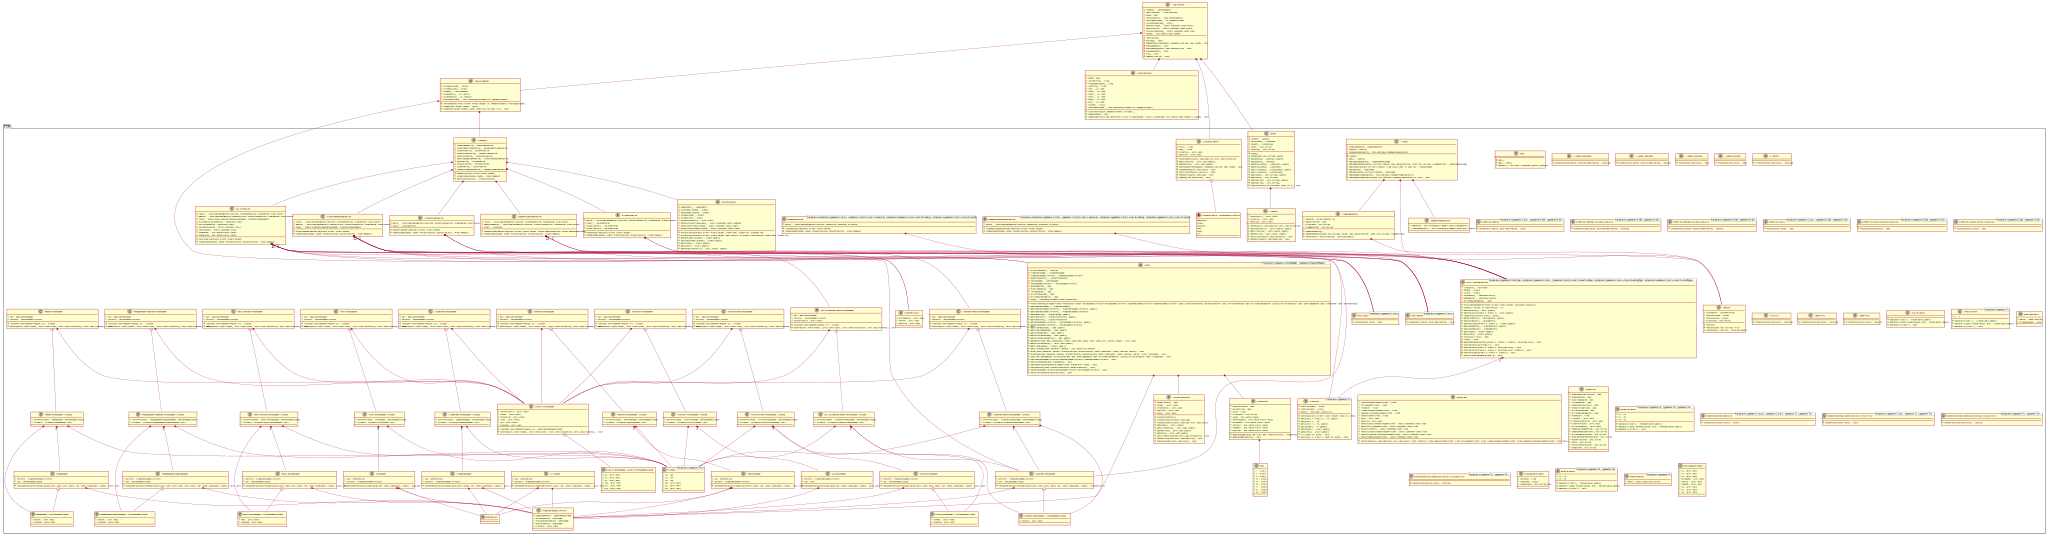
\includegraphics[scale=0.065]{output.eps}
\subsubsection{Легенда и краткое описание элементов диаграммы}
\includegraphics[scale=0.5]{notation_class.jpg}
\includegraphics[scale=0.5]{Uml_classes_en.svg.png}\\
Картинки взяты отсюда ~\cite{uml1} и отсюда ~\cite{uml2}. В источнике ~\cite{uml2} достаточно подробно описывается формат UML, если читатель хочет узнать больше про данный формат.

\subsection{Тесты на производительность}
Время отрисовки кадра сильно зависит от разрешения окна, количества объектов в сцене, площади экрана, покрываемой треугольниками, применяемых шейдеров и выбранного пайплайна отрисовки (стандартный пайплайн, bloom, shadow mapping и т.д.). Ниже приведены времена отрисовки для некоторых сцен. Проверить производительность можно, если запустить сцены с именами ''bench*.scn''. Тестирование производилось на ноутбуке с процессором intel pentium 4415U, 2.3 GHz, 2 физических (4 виртуальных) ядра, окно в разрешении 1200x800.

\begin{center}
\begin{tabular}{|c|c|}
	\hline
	Имя сцены & Время отрисовки кадра, ms \\
	\hline
	bench\_teapot1\_white & 38 \\
	bench\_teapot1\_texture & 44 \\
	bench\_teapot1\_phong & 72 \\
	bench\_teapot1\_phong2 & 85 \\
	bench\_teapot1\_normal & 261 \\
	bench\_teapot1\_disp & 376 \\
	bench\_teapot1\_bloom & 574 \\
	bench\_teapot1\_transparent & 85 \\
	bench\_teapot1\_ssao & 1325 \\
	\hline
\end{tabular}
\end{center}

Описание сцен: 
\begin{itemize}
	\item white - Просто белый чайник, шейдер возвращает константный цвет.
	\item texture - Чайник с текстурой (uv координаты для данной модели генерируются автоматически и имеют мало смысла, эта сцена, как и остальные, нужна просто для проверки производительности).
	\item phong - Blinn-Phong шейдер.
	\item phong2 - То же самое, только 2 источника света.
	\item normal - Normal mapping.
	\item disp - Parallax mapping.
	\item bloom - phong2 + bloom пайплайн (нужно выбрать bloom вместо default пайплайн-а).
	\item transparent - Полупрозрачный чайник (нужно выбрать blending with sort пайплайн).
	\item ssao - чайник с белой текстурой, Blinn-Phong шейдер, источников света нет, SSAO пайплайн (нужно выбрать SSAO вместо default пайплайн-а).
\end{itemize}

Чайник состоит из 6320 треугольников, во всех сценах кроме disp и normal расположен одинаково и занимает примерно треть окна по площади. В сценах disp и normal чайник расположен близко к камере и занимает практически всё пространство окна.

Скриншоты сцен - рис. \ref{fig:bench} (сцены идут по порядку слева направо, сверху вниз):
\begin{SCfigure}[0.5][h]
	\label{fig:bench}
	\caption{Скриншоты сцен, на которых тестировалась производительность.}
	\includegraphics[width=0.6\textwidth]{benchmark.png}
\end{SCfigure}

\section{Заключение}
\subsection{Результат}
Главный результат работы - это интерактивное приложение, позволяющее пользователю взаимодействовать с трёхмерной сценой, задавать различные режимы отрисовки для объектов сцены, менять параметры освещения, источников света, камеры и экрана в реальном времени. 

В 3D рендерере, на базе которого построено приложение, реализованы продвинутые алгоритмы 3D рендеринга: normal mapping, parallax mapping, HDR, bloom, blending (поддержка полупрозрачных объектов), shadow mapping, deferred shading, SSAO. Результаты работы данных алгоритмов, и то, как их применение / неприменение визуально влияет на отрисованную сцену, можно наглядно увидеть с помощью использования приложения. 
\subsubsection{Количественные характеристики (просили привести)}
\begin{itemize}
	\item Число строк кода: 2475 в ''.h'' файлах, 2168 в ''.cpp'' файлах. Итого: 4643 строчки кода. Для подсчёта использовалась команда: \begin{verbatim}find . -name '*.php' | sed 's/.*/"&"/' | xargs  wc -l
	\end{verbatim}
	(вместо php cpp и h)
	\item Объём кода в килобайтах: 147.
	\item Но необходимо учитывать, что данный проект - это продолжение проекта прошлого года, поэтому часть строк уже существовала на момент начала работы над проектом, и частично строки переписывались, рефакторились и т.д. Также здесь в количестве строк учитываются комментарии, пустые строки, строки с фигурными скобками. Поэтому не уверен, что по данной статистике можно сделать какие-то определённые выводы.
\end{itemize}
\subsection{Направления дальнейших разработок}
Как было написано в аннотации, в сфере 3D рендеринга существует множество статей и различных алгоритмов, поэтому дальнейшую разработку можно посвятить реализации ещё не затронутых методов 3D рендеринга. Также всегда можно заняться оптимизацией производительности (хотя аппаратные рендереры всё равно будут значительно эффективнее), улучшению качества кода, и т.д.

\renewcommand{\refname}{Библиографический список}

\bibliographystyle{plainurl}
\bibliography{bibl}



% С этого момента глобальная нумерация идет буквами. Этот раздел я добавил лишь для демонстрации возможностей LaTeX, его можно и нужно удалить и он не нужен для курсового проекта непосредственно.
%\appendix

%Проведем небольшой обзор возможностей \LaTeX. Далее идет обзорный кусок, который надо будет вырезать. Он приведен лишь для демонстрации возможностей \LaTeX.

%\section{Нумеруемый заголовок}
%Текст раздела
%\subsection{Нумеруемый подзаголовок}
%Текст подраздела
%\subsubsection{Нумеруемый подподзаголовок}
%Текст подподраздела

%\section*{Не нумеруемый заголовок}
%Текст раздела
%\subsection*{Не нумеруемый подзаголовок}
%Текст подраздела
%\subsubsection*{Не нумеруемый подподзаголовок}
%Текст подподраздела


%\paragraph{Заголовок абзаца} Текст абзаца

%Формулы в тексте набирают так $x = e^{\pi i}\sqrt{\text{формула}}$. Выключенные не нумерованные формулы набираются либо так:
%\[
%x = e^{\pi i}\sqrt{\text{формула}}
%\]
%Либо так
%$$
%x = e^{\pi i}\sqrt{\text{формула}}
%$$
%Первый способ предпочтительнее при подаче статей в журналы AMS, потому рекомендую привыкать к нему.

%Выключенные нумерованные формулы:
%\begin{equation}\label{Equation1}
% \label{имя-метки} эта команда ставит метку, на которую потом можно сослаться с помощью \ref{имя-метки}. Метки можно ставить на все объекты, у которых есть автоматические счетчики (номера разделов, подразделов, теорем, лемм, формул и т.д.
%x = e^{\pi i}\sqrt{\text{формула}}
%\end{equation}
%Или не нумерованная версия
%\begin{equation*}
%x = e^{\pi i}\sqrt{\text{формула}}
%\end{equation*}

%Уравнение~\ref{Equation1} радостно занумеровано.

%Лесенка для длинных формул
%\begin{multline}
%x = e^{\pi i}\sqrt{\text{очень очень очень длинная формула}}=\\
%\tr A - \sin(\text{еще одна очень очень длинная формула})=\\
%\cos z \Im \varphi(\text{и последняя длинная при длинная формула})
%\end{multline}

%Многострочная формула с центровкой
%\begin{gather}
%x = e^{\pi i}\sqrt{\text{очень очень очень длинная формула}}=\\
%\tr A - \sin(\text{еще одна очень очень длинная формула})=\\
%\cos z \Im \varphi(\text{и последняя длинная при длинная формула})
%\end{gather}

%Многострочная формула с ручным выравниванием. Выравнивание идет по знаку $\&$, который на печать не выводится.
%\begin{align}
%x = &e^{\pi i}\sqrt{\text{очень очень очень длинная формула}}=\\
%&\tr A - \sin(\text{еще одна очень очень длинная формула})=\\
%&\cos z \Im \varphi(\text{и последняя длинная при длинная формула})
%\end{align}

%\begin{theorem}
%Текст теоремы
%\end{theorem}
%\begin{proof}
%В специальном окружении оформляется доказательство.
%\end{proof}

%\begin{theorem}[Имя теоремы]
%Текст теоремы
%\end{theorem}
%\begin{proof}[Доказательство нашей теоремы]
%В специальном окружении оформляется доказательство.
%\end{proof}

%\begin{definition}
%Текст определения
%\end{definition}

%\begin{remark}
%Текст замечания
%\end{remark}

%\paragraph{Перечни:} Нумерованные
%\begin{enumerate}
%\item Первый
%\item Второй
%\begin{enumerate}
%\item Вложенный первый
%\item Вложенный второй
%\end{enumerate}
%\end{enumerate}

%Не нумерованные

%\begin{itemize}
%\item Первый
%\item Второй
%\begin{itemize}
%\item Вложенный первый
%\item Вложенный второй
%\end{itemize}
%\end{itemize}


% Здесь текст документа заканчивается
\end{document}
% Начиная с этого момента весь текст LaTeX игнорирует, можете вставлять любую абракадабру.
